\PassOptionsToPackage{unicode=true}{hyperref} % options for packages loaded elsewhere
\PassOptionsToPackage{hyphens}{url}
%
\documentclass[]{book}
\usepackage{lmodern}
\usepackage{amssymb,amsmath}
\usepackage{ifxetex,ifluatex}
\usepackage{fixltx2e} % provides \textsubscript
\ifnum 0\ifxetex 1\fi\ifluatex 1\fi=0 % if pdftex
  \usepackage[T1]{fontenc}
  \usepackage[utf8]{inputenc}
  \usepackage{textcomp} % provides euro and other symbols
\else % if luatex or xelatex
  \usepackage{unicode-math}
  \defaultfontfeatures{Ligatures=TeX,Scale=MatchLowercase}
\fi
% use upquote if available, for straight quotes in verbatim environments
\IfFileExists{upquote.sty}{\usepackage{upquote}}{}
% use microtype if available
\IfFileExists{microtype.sty}{%
\usepackage[]{microtype}
\UseMicrotypeSet[protrusion]{basicmath} % disable protrusion for tt fonts
}{}
\IfFileExists{parskip.sty}{%
\usepackage{parskip}
}{% else
\setlength{\parindent}{0pt}
\setlength{\parskip}{6pt plus 2pt minus 1pt}
}
\usepackage{hyperref}
\hypersetup{
            pdftitle={Reproducible Medical Research with R},
            pdfauthor={Peter D.R. Higgins, MD, PhD, MSc},
            pdfborder={0 0 0},
            breaklinks=true}
\urlstyle{same}  % don't use monospace font for urls
\usepackage{longtable,booktabs}
% Fix footnotes in tables (requires footnote package)
\IfFileExists{footnote.sty}{\usepackage{footnote}\makesavenoteenv{longtable}}{}
\usepackage{graphicx,grffile}
\makeatletter
\def\maxwidth{\ifdim\Gin@nat@width>\linewidth\linewidth\else\Gin@nat@width\fi}
\def\maxheight{\ifdim\Gin@nat@height>\textheight\textheight\else\Gin@nat@height\fi}
\makeatother
% Scale images if necessary, so that they will not overflow the page
% margins by default, and it is still possible to overwrite the defaults
% using explicit options in \includegraphics[width, height, ...]{}
\setkeys{Gin}{width=\maxwidth,height=\maxheight,keepaspectratio}
\setlength{\emergencystretch}{3em}  % prevent overfull lines
\providecommand{\tightlist}{%
  \setlength{\itemsep}{0pt}\setlength{\parskip}{0pt}}
\setcounter{secnumdepth}{5}
% Redefines (sub)paragraphs to behave more like sections
\ifx\paragraph\undefined\else
\let\oldparagraph\paragraph
\renewcommand{\paragraph}[1]{\oldparagraph{#1}\mbox{}}
\fi
\ifx\subparagraph\undefined\else
\let\oldsubparagraph\subparagraph
\renewcommand{\subparagraph}[1]{\oldsubparagraph{#1}\mbox{}}
\fi

% set default figure placement to htbp
\makeatletter
\def\fps@figure{htbp}
\makeatother

\usepackage{booktabs}
\usepackage{amsthm}
\makeatletter
\def\thm@space@setup{%
  \thm@preskip=8pt plus 2pt minus 4pt
  \thm@postskip=\thm@preskip
}
\makeatother
\usepackage[]{natbib}
\bibliographystyle{apalike}

\title{Reproducible Medical Research with R}
\author{Peter D.R. Higgins, MD, PhD, MSc}
\date{2020-04-15}

\begin{document}
\maketitle

{
\setcounter{tocdepth}{1}
\tableofcontents
}
\hypertarget{preface}{%
\chapter{Preface}\label{preface}}

Welcome to Reproducible Medical Research with R (RMWR). I hope that this book meets your needs.

\hypertarget{who-this-book-is-for}{%
\section{Who This Book is For}\label{who-this-book-is-for}}

This is a book for anyone in the medical field interested in analyzing the data available to them to better understand health, disease, or delivery of care. This could include nurses, dieticians, psychologists, and PhDs in related fields, as well as medical students, residents, fellows, or doctors in practice.\\
I expect that most learners will be using this book in their spare time at night and on weekends, as the medical school curriculum is already packed full, and there is no room to add skills in reproducible research to the standard curriculum. This book is designed for self-teaching, and many hints and solutions will be provided to avoid roadblocks and frustration.
Many learners find themselves wanting to develop reproducible research skills after they have finished their training, and after they have become comfortable with their clinical role. This is the time when they identify and want to address problems in their practice with the data they have before them. This book is for you.

\hypertarget{the-spiral-of-success-structure}{%
\section{The Spiral of Success Structure}\label{the-spiral-of-success-structure}}

This book is structured on the concept of a ``spiral of success'', with readers learning about topics like data visualization, data wrangling, data modeling, reproducible research, and communication of results in repeated passes. These will initially be at a superficial level, and at each pass of the spiral, will provide increasing depth and complexity. This means that the chapters on data wrangling will not all be together, nor the chapters on data visualization. Our goal is to build skills gradually, and return to (and remind students of) their previously built skills in one area and to add to them. The eventual goal is for learners to be able to produce, document, and communicate reproducible research to their community.

\hypertarget{motivation-for-this-book}{%
\section{Motivation for this Book}\label{motivation-for-this-book}}

Most medical people who learn R to do their own data analysis do it on their own time. They rarely have time for a semester-long course, and their clinical schedules usually will not allow it. Fortunately, a lot of people learn R on their own, and there is a strong and supportive R Community to help new learners. A 2019 Twitter survey conducted by \texttt{@RLadies} found that more than half of respondents were largely self-taught, from books and online resources.

There are a lot of good resources for learning R, so why one more? In part, because the needs of a medical audience are often different. There are distinct needs for protecting health information, generating a descriptive Table One, using secure data tools like REDCap, and creating standard medical journal and meeting output in Word, Powerpoint, and poster formats.

More and more, all science is becoming data science. We are able to track patients, their test results, and even the individual pixels (voxels) of their CT scans electronically, and use those data points to develop new knowledge. While one could argue that health care workers should collect data and bring it to trained statisticians, this does not work nearly as well as you might expect. Most academic statisticians are incentivized to develop new statistical methods, and are not very interested (or incentivized) to do the hand-holding required to wrangle messy clinical data into a manuscript.

There also are simply not enough statisticians to meet the needs of medical science. Having clinicians on the front lines with some data science training makes a big difference, whether in 1854 in London (John Snow) or in 2014 in Flint, Michigan (Mona Hanna-Atisha). Having more clinicians with some training will impact medical care, as they will identify local problems that would have otherwise never reached a statistician, and probably never been addressed with data otherwise.

\hypertarget{the-scientific-reproducibility-crisis}{%
\section{The Scientific Reproducibility Crisis}\label{the-scientific-reproducibility-crisis}}

Beginning as far back as 1989, with the David Baltimore case, and increasingly publicly through the 2010s, there has been a rising tide of realization that a lot of taxpayer-funded science is done sloppily, and that our standards as scientists need to be higher. The line between carelessly-done science and outright fraud is a thin one, and the case can be made that doing science in a sloppy fashion defrauds the funders, as it leads to results that can not be reproduced nor replicated. Particularly in medicine, where incorrect findings can cause great harm, we should take special care to do scientific research which is well-documented, reproducible, and replicable. This topic as a motivating force for doing careful medical research will be expanded upon in Chapter 1.

\hypertarget{what-this-book-is-not}{%
\section{What this Book is Not}\label{what-this-book-is-not}}

\hypertarget{this-book-is-not-a-statistics-text}{%
\subsection{This Book is Not A Statistics Text}\label{this-book-is-not-a-statistics-text}}

This is not an introduction to statistics. I am assuming that you have learned some statistics somewhere in secondary school, undergraduate studies, graduate school, or even medical school. There are lots of statisticians with Ph.D.s who can certainly teach statistics much more effectively than I can. While I have a master's degree in Clinical Research Design and Statistical Analysis (isn't that a mouthful!) from the University of Michigan, I will leave formal teaching of statistics to the pros.

If you need to brush up on your statistics, no worries. There are several excellent (and free!) e-books on that very topic, using R. Some good examples include (go ahead and click through the blue links to explore):

\begin{enumerate}
\def\labelenumi{\arabic{enumi}.}
\tightlist
\item
  \href{https://learningstatisticswithr-bookdown.netlify.com}{Learning Statistics with R (LSR)}
\item
  \href{https://bookdown.org/fjmcgrade/ismaykim/}{Modern Dive}
\item
  \href{https://tinystats.github.io/teacups-giraffes-and-statistics/index.html}{Teacup Giraffes}
\end{enumerate}

We will cover a lot of the same materials as these books, but with a less theoretical and more applied approach. I will focus on specific medical examples, and emphasize issues (like Protected Health Information) that are particularly important for medical data. I am assuming that you are here because you want to analyze your own data in your probably very limited free time.

\hypertarget{this-book-does-not-provide-comprehensive-coverage-of-the-r-universe}{%
\subsection{This Book Does Not Provide Comprehensive Coverage of the R Universe}\label{this-book-does-not-provide-comprehensive-coverage-of-the-r-universe}}

This book is also far from comprehensive in teaching what is available in the R ecosystem. This book should be considered a launch pad. Many of the later chapters will give you a taste of what is available in certain areas, and guide you to resources (and links) that you can explore to learn more and do more beyond the scope of this book.

\hypertarget{some-guideposts}{%
\section{Some Guideposts}\label{some-guideposts}}

Keep an eye out for Guideposts, which look like this:

\textbf{Warnings}

This is a common gotcha. Watch out for this.

\textbf{Tips}

This is a helpful tip for debugging.

\textbf{Try It Out}

Take what you have learned and try it yourself in the code box below.

\textbf{Challenge} - take the next step and try a more challenging example.

Try this more complicated example.

\textbf{Explore More} - resources for learning more about a particular topic.

If you want to learn more about Shiny apps, go to \url{https://mastering-shiny.org} to see an entire book on the topic.

\hypertarget{getting-started-and-installing-your-tools}{%
\chapter{Getting Started and Installing Your Tools}\label{getting-started-and-installing-your-tools}}

One of the most intimidating parts of getting started with something new is the actual getting started part. Don't worry, we will walk you through this step-by step.

\hypertarget{goals-for-this-chapter}{%
\section{Goals for this Chapter}\label{goals-for-this-chapter}}

\begin{itemize}
\tightlist
\item
  Install R on your Computer
\item
  Install RStudio on your Computer
\item
  Install Git on your Computer
\item
  Get Acquainted with the RStudio IDE
\end{itemize}

\hypertarget{website-links-needed-for-this-chapter}{%
\section{Website links needed for this Chapter}\label{website-links-needed-for-this-chapter}}

While in many chapters, we will list the R packages you need, in this chapter, you will be downloading and installing new software, so we will list the links here for your reference

\begin{itemize}
\tightlist
\item
  \url{https://www.r-project.org}
\item
  \url{https://rstudio.com/products/rstudio/download/}
\item
  \url{https://git-scm.com/downloads}
\end{itemize}

\hypertarget{pathway-for-this-chapter}{%
\section{Pathway for this Chapter}\label{pathway-for-this-chapter}}

This Chapter is part of the \textbf{TOOLS} pathway.
Chapters in this pathway include

\begin{itemize}
\tightlist
\item
  Getting Started and Installing Your Tools
\item
  Updating R, RStudio, and Your Packages
\item
  Advanced Use of the RStudio IDE
\item
  When You Don't Want to Update Packages (Using \emph{renv})
\item
  Major R Updates (Where Are My Packages?)
\end{itemize}

\hypertarget{installing-r-on-your-computer}{%
\section{Installing R on your Computer}\label{installing-r-on-your-computer}}

\hypertarget{installing-rstudio-on-your-computer}{%
\section{Installing RStudio on your Computer}\label{installing-rstudio-on-your-computer}}

\hypertarget{installing-git-on-your-computer}{%
\section{Installing Git on your Computer}\label{installing-git-on-your-computer}}

\hypertarget{getting-acquainted-with-the-rstudio-ide}{%
\section{Getting Acquainted with the RStudio IDE}\label{getting-acquainted-with-the-rstudio-ide}}

\hypertarget{a-tasting-menu-of-r}{%
\chapter{A Tasting Menu of R}\label{a-tasting-menu-of-r}}

In this chapter, we will introduce you to a lot of neat things that you can do with R and RStudio, and you will publish a simple data analysis on the Internet
that you can share with friends and family.

\hypertarget{setting-the-table}{%
\section{Setting the Table}\label{setting-the-table}}

At the end of this chapter, you will publish a data analysis to \emph{RPubs}, a free website site where you can share your data analyses and visualizations. First you will need to set up an account on RPubs. Start by opening a new tab in your browser, and navigating to this \href{https://rpubs.com/users/new}{RPubs link}. It should look like the image below.
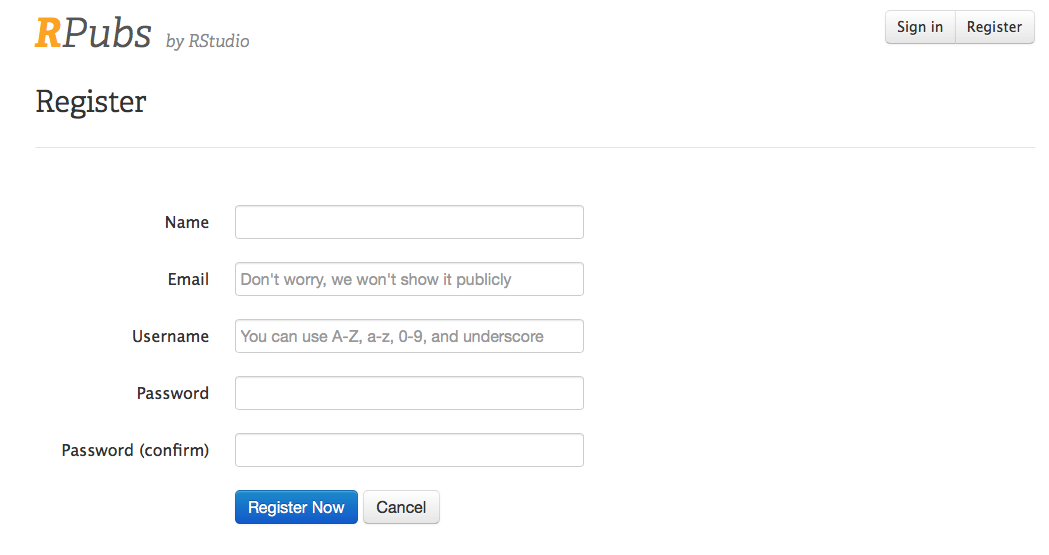
\includegraphics{images/rpubs1.png}\\
Enter your name, email, username and password, and click on the \emph{Register Now} button, and you will be set up to use RPubs.\\
This will bring you to this page. In the image below, we have set up an account for pdr.\\
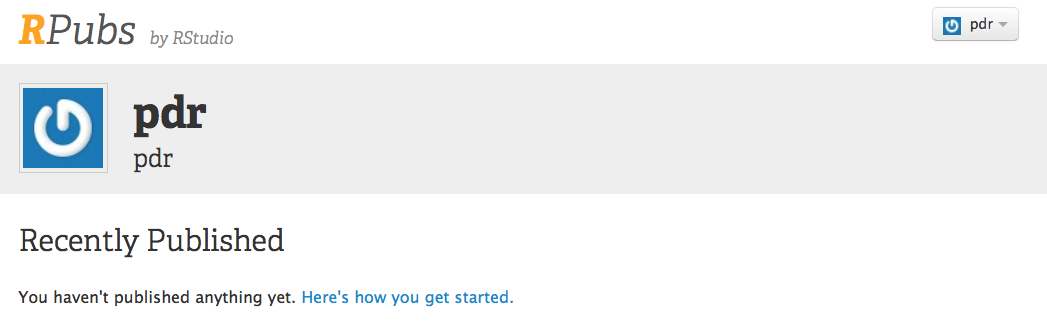
\includegraphics{images/rpubs2.png}
Click on the \emph{Here's How You Get Started} link.
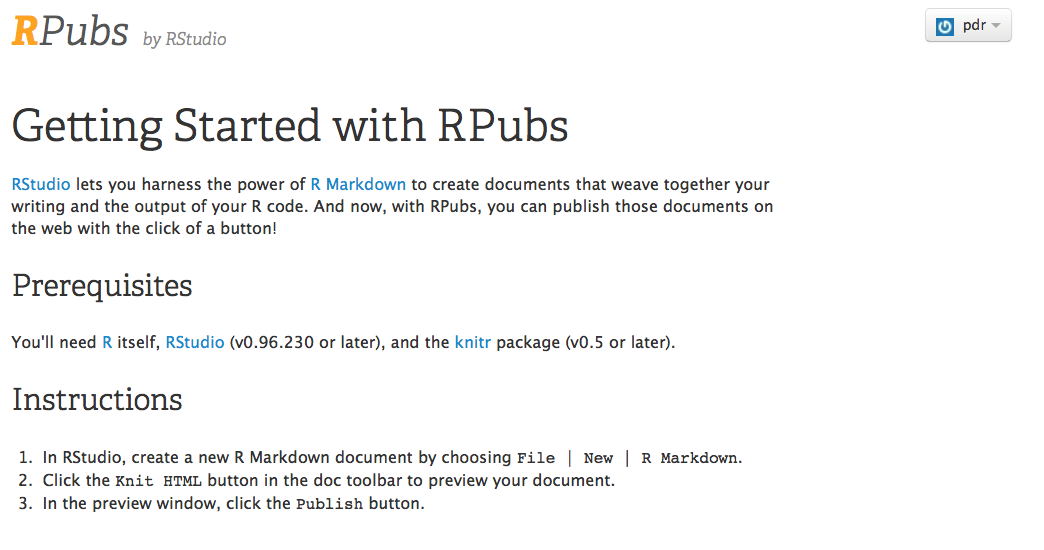
\includegraphics{images/rpubs3.png}\\
You are now all set up and ready to go. Now you have a place on the internet to share your R creations!

\hypertarget{goals-for-this-chapter-1}{%
\section{Goals for this Chapter}\label{goals-for-this-chapter-1}}

\begin{itemize}
\tightlist
\item
  Open a New Rmarkdown document
\item
  Read in Data from a file
\item
  Wrangle Your Data
\item
  Visualize Your Data
\item
  Publish your work to RPubs
\item
  Check out Interactive Plots
\item
  Check out Animated Graphics
\item
  Check out a Clinical Trial Dashboard
\item
  Check out a Shiny App
\end{itemize}

\hypertarget{packages-needed-for-this-chapter}{%
\section{Packages needed for this Chapter}\label{packages-needed-for-this-chapter}}

You will need to enter this line of code into your console, to make sure that the tidyverse package is installed on your computer.
\texttt{install.packages("tidyverse")}

In the setup chunk of your Rmarkdown document, you will need to access the tidyverse package with one line of code:
\texttt{library(tidyverse)}

\hypertarget{website-links-needed-for-this-chapter-1}{%
\section{Website links needed for this Chapter}\label{website-links-needed-for-this-chapter-1}}

In this chapter, you will need to access the RPubs website.\\
- \url{https://rpubs.com/}

\hypertarget{pathway-for-this-chapter-1}{%
\section{Pathway for this Chapter}\label{pathway-for-this-chapter-1}}

This Chapter is part of the \textbf{XXX} pathway.
Chapters in this pathway include

\hypertarget{open-a-new-rmarkdown-document}{%
\section{Open a New Rmarkdown document}\label{open-a-new-rmarkdown-document}}

Let's get started in R. Turn on your computer, and open the RStudio application. You should see the familiar panes for the Console, Environment, and Files.\\
You need to open up a new document to activate the Source pane. While in RStudio, click on File/New File/R Script.
It should look like this.\\
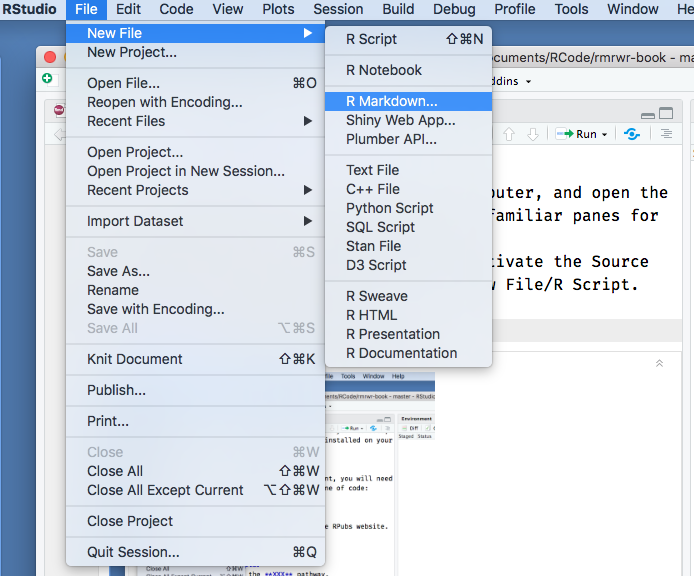
\includegraphics{images/newrmd1.png}
Now you will see the window below. Rename the document from ``Untitled'' to ``Tasting'', and click the OK button.
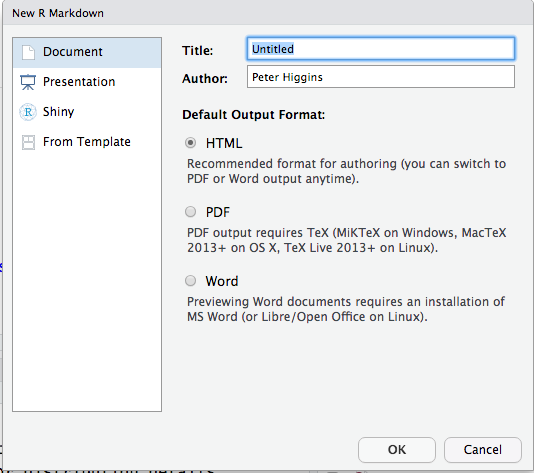
\includegraphics{images/newrmd2.png}

Now the file is open, and looks like the window below. Click on the save icon (like a floppy disk in the top left), and save this document as tasting.Rmd.
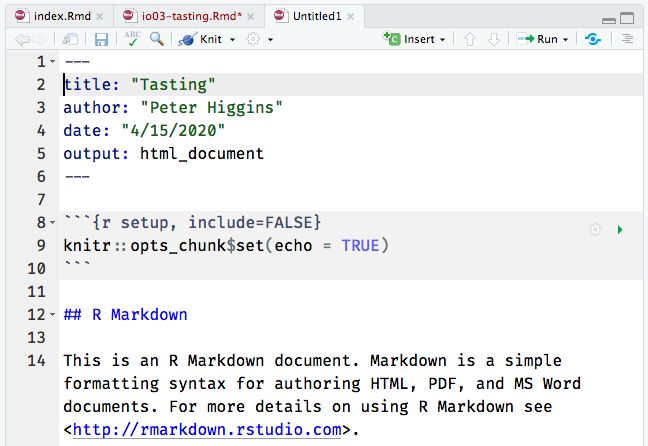
\includegraphics{images/newrmd3.png}
You have created a new Rmarkdown document. An Rmarkdown document lets you mix data, code, and descriptive text. It is very helpful for presenting and explaining data and visualizations. An Rmarkdown document can be converted (Knit) to HTML for a web page, Microsoft Word, Powerpoint, PDF, and several other formats.\\
Code chunks are in a gray color, and both start and end with 3 backticks (````\texttt{).\ \ \ \ \ Text\ can\ be\ body\ text,\ or\ can\ be\ headers\ and\ titles.\ The\ number\ of\ hashtags\ before\ some\ header\ text\ defines\ what\ level\ the\ header\ is.\ \ \ \ \ \ You\ can\ insert\ links,\ pictures,\ and\ YouTube\ videos\ into\ Rmarkdown\ documents\ if\ it\ is\ helpful\ to\ explain\ your\ point.\ \textless{}br\textgreater{}\ The\ first\ code\ chunk\ in\ each\ Rmarkdown\ document\ is\ named}setup\texttt{.\ The\ name\ comes\ after\ the\ left\ curly\ brace\ and\ the\ r\ (}\{r\texttt{)\ at\ the\ beginning\ of\ the\ setup\ chunk.\ The\ letter}r\texttt{tells\ RStudio\ that\ what\ is\ coming\ on\ the\ next\ line\ is\ R\ code\ (RStudio\ can\ also\ use\ SQL,\ C++,\ python,\ and\ several\ other\ languages).\ After\ the\ comma,\ you\ can\ define\ options\ for\ this\ code\ chunk.\ In\ this\ case,\ the\ option}include` is set to FALSE, so that when this Rmarkdown document is knitted, this code chunk will not appear.

\hypertarget{read-in-data-from-a-file}{%
\section{Read in Data from a file}\label{read-in-data-from-a-file}}

\hypertarget{wrangle-your-data}{%
\section{Wrangle Your Data}\label{wrangle-your-data}}

\hypertarget{visualize-your-data}{%
\section{Visualize Your Data}\label{visualize-your-data}}

\hypertarget{publish-your-work-to-rpubs}{%
\section{Publish your work to RPubs}\label{publish-your-work-to-rpubs}}

\hypertarget{the-dessert-cart}{%
\section{The Dessert Cart}\label{the-dessert-cart}}

Below are some examples of neat things you can do with medical data in R. These are more advanced approaches, but completely doable when you have more experience with R.

\hypertarget{interactive-plots}{%
\subsection{Interactive Plots}\label{interactive-plots}}

\hypertarget{animated-graphics}{%
\subsection{Animated Graphics}\label{animated-graphics}}

\hypertarget{a-clinical-trial-dashboard}{%
\subsection{A Clinical Trial Dashboard}\label{a-clinical-trial-dashboard}}

\hypertarget{a-shiny-app}{%
\subsection{A Shiny App}\label{a-shiny-app}}

\hypertarget{an-example-of-synergy-in-the-r-community}{%
\subsection{An Example of Synergy in the R Community}\label{an-example-of-synergy-in-the-r-community}}

One of the remarkable things about the open source R community is that people build all kinds of new R functions and packages that are useful to them, and then share them publicly with tools like \emph{Github} so that they can be useful to others. Often combining bits of several packages leads to \textbf{emergent properties} - completely new creations that can only occur because all of the parts (packages) are present. The collaborative nature of the R community, in this case on Twitter (follow the \#rstats hashtag), can lead to surprising collaborations and outcomes.\\
See the example below.\\
Go ahead, \emph{click} on the play button to run the gifs. All coded in R.\\

I used a modified version of \citet{djnavarro}'s flametree package to produce this fractal tree in 3D, placed it in a LEGO planter for \citet{ryantimpe}, set down a copy of \citet{skyetetra} and \citet{robinson_es}'s book for some light reading, and of course, used \#rayrender and \#rstats to render it all :) https://t.co/qRg2omUftw pic.twitter.com/Ff9VeLtX97

--- Tyler Morgan-Wall (\citet{tylermorganwall}) April 14, 2020

\hypertarget{updating-r-rstudio-and-your-packages}{%
\chapter{Updating R, RStudio, and Your Packages}\label{updating-r-rstudio-and-your-packages}}

This is an R Markdown document. Markdown is a simple formatting syntax for authoring HTML, PDF, and MS Word documents. For more details on using R Markdown see \url{http://rmarkdown.rstudio.com}.

\hypertarget{major-r-updates-where-are-my-packages}{%
\chapter{Major R Updates (Where Are My Packages?)}\label{major-r-updates-where-are-my-packages}}

This is an R Markdown document. Markdown is a simple formatting syntax for authoring HTML, PDF, and MS Word documents. For more details on using R Markdown see \url{http://rmarkdown.rstudio.com}.

\hypertarget{time-series-data-with-the-tidyverts-packages}{%
\chapter{Time Series data with the Tidyverts Packages}\label{time-series-data-with-the-tidyverts-packages}}

Fun text here.
All kinds of crazy examples.
Time series with data from influenza pandemic of 1918-19, perhaps.
This is a book for anyone in the medical field interested in analyzing the data available to them to better understand health, disease, or delivery of care. This could include nurses, dieticians, psychologists, and PhDs in related fields, as well as medical students, residents, fellows, or doctors in practice.\\
I expect that most learners will be using this book in their spare time at night and on weekends, as the medical school curriculum is already packed full, and there is no room to add skills in reproducible research to the standard curriculum. This book is designed for self-teaching, and many hints and solutions will be provided to avoid roadblocks and frustration.

\hypertarget{tsibble}{%
\section{Tsibble}\label{tsibble}}

Time series tibble

\href{https://tidyverts.org}{Tidyverts webpage}

\hypertarget{fable}{%
\section{Fable}\label{fable}}

Tidy forecasting

\hypertarget{feasts}{%
\section{Feasts}\label{feasts}}

Feature extraction and Statistics

\hypertarget{slider}{%
\section{Slider}\label{slider}}

Rolling anaylsis with window functions.\\
\href{https://davisvaughan.github.io/slider/}{Slider packagedown page}

\bibliography{book.bib,packages.bib}

\end{document}
